A mount was designed and fabricated to house the cameras and triggering electronics so that it could be mounted to a X8 UAV platform.  The constraints and goals of the design were as follows:
\begin{itemize}
	\item Weigh under 800g (X8 payload limit)
	\item House 4 GoPro cameras and triggering electronics
	\item Rigid, to ensure constant relative orientations between the cameras
	\item Easily manufactured for rapid prototyping and improvements
	\item Designed so cameras and electronics can be easily removed
	\item Little to no tools required
	\item Low cost 
\end{itemize}
\section{3D CAD Design}
Given the design constraints, it was clear that 3D printing using PLA or ABS plastic provided the most robust manufacturing methodology. The plastic is lightweight, easily manufactured, perfect for rapid prototyping, low cost, rigid, and can be designed with intricate interlocking parts to minimize the use of tools.  Each part of the sensor that was 3D printed was designed for 3D printing to minimize the amount of support required.  Each part has an optimal orientation that it should be printed at, so as to maximize structural integrity and minimize support. For example, a five sided hollow cube should be printed so that the open face is up, so that no support is necessary.  The orientation of each of the parts should be intuitive to the user.
	\subsection{Camera Enclosure Design}
	The GoPro camera enclosure, shown in \figref{fig:camEnclosure} was designed so that the cameras could be easily removed, as well as fit tightly into the enclosure so that there is no movement or shifting during the flight.  Many prototypes were generated, and various tolerances were investigated to ensure a compromise of ``easy to remove'' and ``doesn't move while in flight.''  A hinged design was selected as it minimized the number of screws or tools required, and was also a simple design to 3D print.  The lens protrudes into the threaded cylinder on the lid, and all of the ports and buttons are accessible.  The enclosure consists of 3 parts:
	\begin{enumerate}
		\item Enclosure (yellow): This is the main body that the GoPro mounts into
		\item Lid (red): This is the hinged part that locks the camera into place
		\item Cap (not shown): This 3D printed part threads onto the lid to protect the GoPro lens when the cameras is not acquiring imagery.
	\end{enumerate}
	The lid and cap are printed individually, while the enclosure is mounted to the Camera Mount in software, and printed as a fused, solid part, as shown in \figref{fig:mountcombo}.
	\begin{figure}[H]
		\centering
		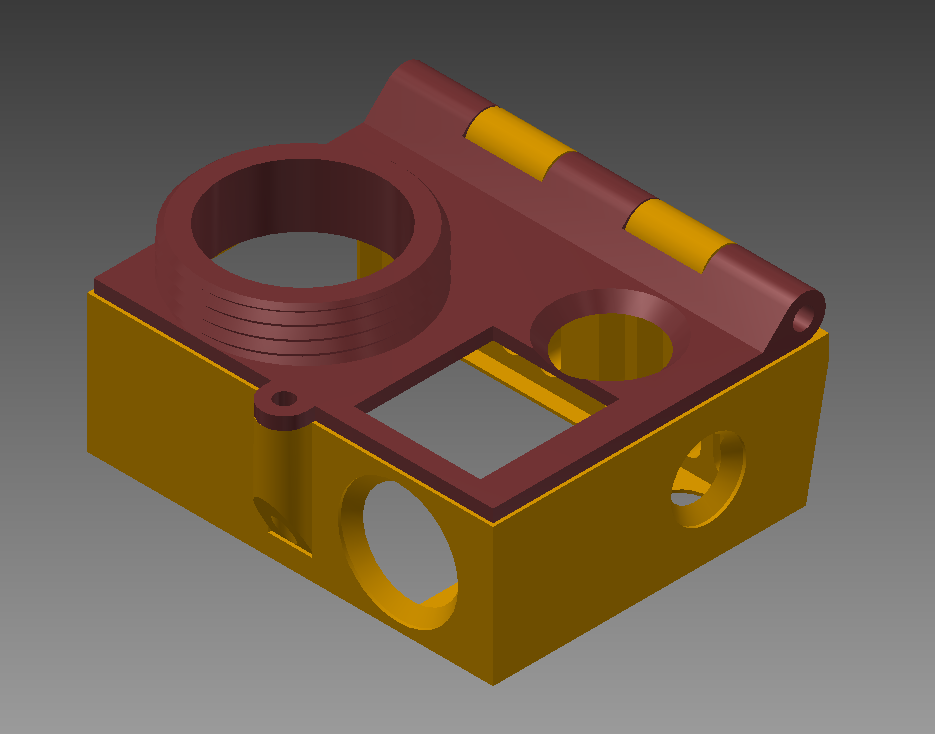
\includegraphics[scale = 0.4]{../figures/cad/cameraEnclosure.png}
		\caption{The camera enclosure was designed with a hinge, and one locking screw.  The threaded area around the cylinder for the lens enables a protective cap to be screwed on.}
		\label{fig:camEnclosure}
	\end{figure}

	\subsection{Camera Mount Design}
	The camera mount, shown in \figref{fig:mount}, defines the orientation of each of the cameras, and is the main frame of the design.  The camera enclosures are mounted directly to each of the four bottom planes in software, and together they are printed as one piece.  This print requires some support material to be removed, but ensures less tools and moving parts in the final design.  The proper orientation for printing the Camera Mount is with the wide opening for the electronics tray facing upwards, so that no support material is required within the body.

	The camera mount is designed so that the electronics tray can slide in and out such that the triggering electronics may be removed easily.  It also incorporates a honeycomb pattern on the top to reduce the overall weight of the system.  The four legs are designed so that vibration damping balls may be placed to connect the system to the X8 Quadcopter legs, shown in \figref{fig:legs}.  
	\begin{figure}[H]
		\centering
		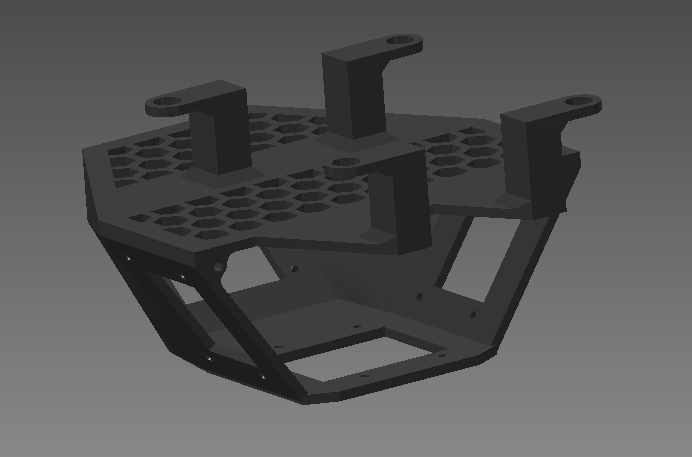
\includegraphics[scale = 0.4]{../figures/cad/mount.png}
		\caption{The camera mount was designed separately from the enclosure, so that the 4 cameras could be mounted to the design in software and they could be printed as one part.}
		\label{fig:mount}
	\end{figure}
	
	\subsection{Electronics Tray and Panel}
	The electronics tray, shown in \figref{fig:elec}, was designed for easy access to the electronics PCB, while still providing status lights and a power switch on the outside.  The tray is locked in with two screws in the upper corners, to ensure it does not slide out during a flight.  The panel portion of the tray, houses three status LEDs, a Voltage LCD display, a power switch, the panel PCB for connections, and an external antenna connection point.  The decoupling of the electronics tray from the mount allows for various electronics packages and batteries to be integrated into the system, without having to redesign a new mount.
	\begin{figure}[H]
		\centering
		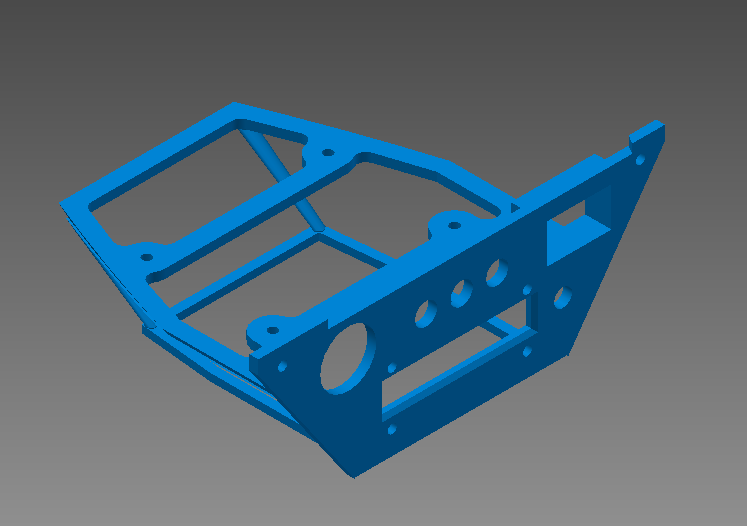
\includegraphics[scale = 0.4]{../figures/cad/electronicsTray.png}
		\caption{The electronics tray was designed so that the PCBs could easily be slid in and out, while the panel provided power and status lights.}
		\label{fig:elec}
	\end{figure}
		
	\subsection{X8 Quadcopter Legs Design}
	The X8 legs mount to the X8 chassis using three bolts.  These straddle the battery, and provide a socket for the vibration damping balls to be attached to.  These vibration damping balls, shown in \figref{fig:vibballs}, are integrated to reduce the propagation of vibration from the motors to the cameras.  Both 200g and 300g vibration damping balls were provided, as the optimum type has not been determined.  Based on the weight of the system, four 200g vibration damping balls should provide a good initial amount of vibration damping. 
	\begin{figure}[H]
		\centering
		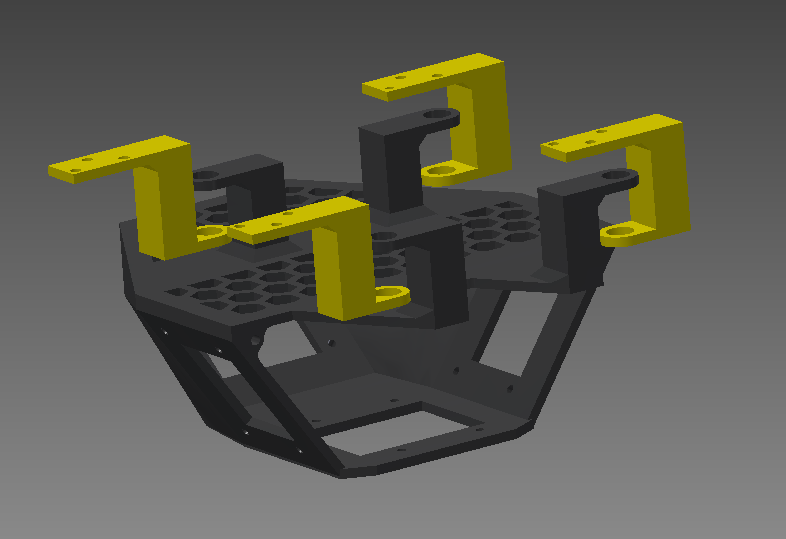
\includegraphics[scale = 0.4]{../figures/cad/bracket.png}
		\caption{The X8 legs were designed so that a vibration damping ball could be placed in between the legs to reduce vibration.}
		\label{fig:legs}
	\end{figure}

	\begin{figure}[H]
		\centering
		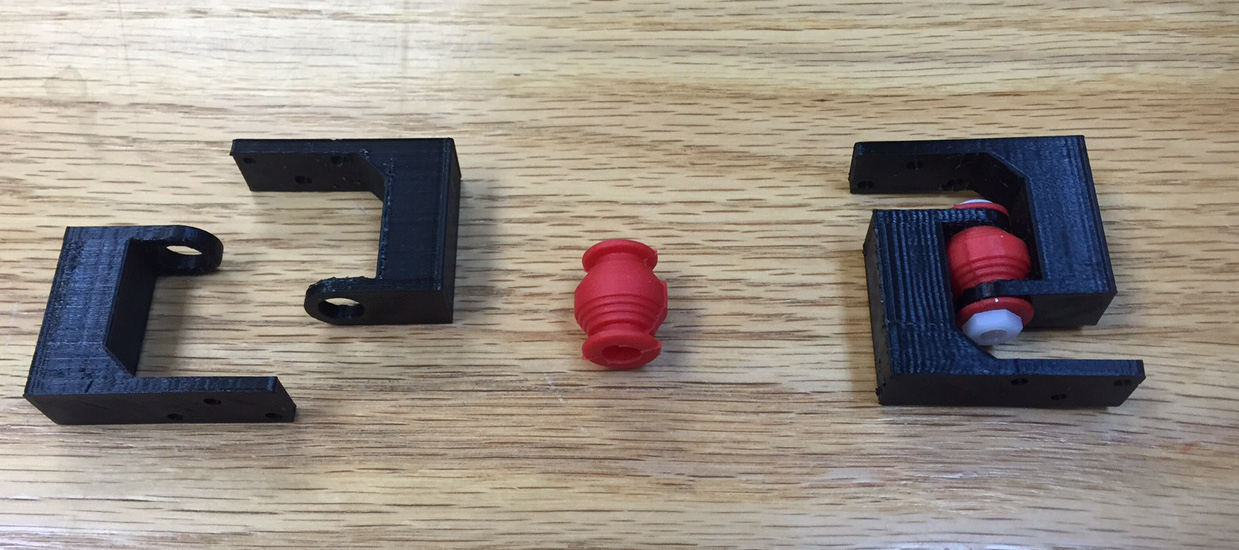
\includegraphics[scale = 0.25]{../figures/vibballs.JPG}
		\caption{The vibration damping balls, shown in red, are used to connect the X8 to the mount and reduce the vibration from the X8 motors.}
		\label{fig:vibballs}
	\end{figure}
	\section{Full Design Specs}
	The final system weighs ~700g with all of the cameras and electronics on board, and can be printed with one 1kg spool of printer filament.  The full system, shown in \figref{fig:mountcombo} is mounted to the X8 and can acquire imagery for approximately 15 minutes.  The fully mounted system is shown in \figref{fig:x8mounted}.  
	
	\begin{figure}[H]
		\centering
		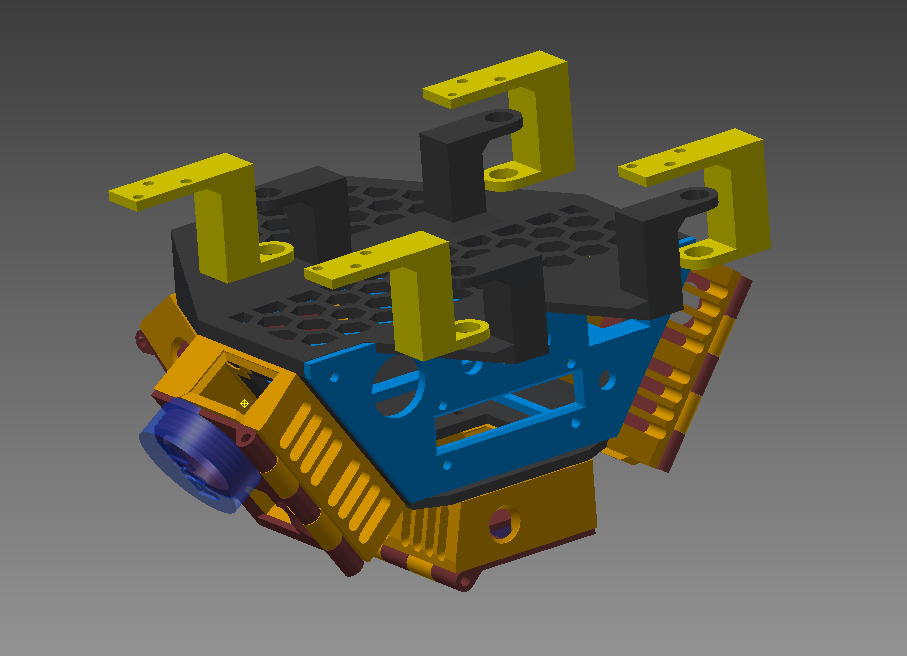
\includegraphics[scale = 0.4]{../figures/cad/all.png}
		\caption{The camera mount was designed separately from the enclosure, so that the 4 cameras could be mounted to the design in software and they could be printed as one part.}
		\label{fig:mountcombo}
	\end{figure}

	\begin{figure}[H]
		\centering
		\includegraphics[scale = 0.7]{../figures/mvssv2.jpg}
		\caption{The sensor is mounted to the bottom of the X8 with the GoPros installed for a proof of concept flight.}
		\label{fig:x8mounted}
	\end{figure}
	
	\section{Camera Orientations}
	One of the main benefits of the 3D printed CAD Design, is the relative orientations between the cameras can be measured in software.  Although there are sure to be uncertainties with printing and camera placement, the measured orientations should be very accurate.  In order to define the coordinate systems, a central `Mount coordinate system' is defined to align with the X8 body at approximately the center of the mount, as shown in \figref{fig:orient}.  The camera is defined such that the focal point of the camera is the origin, Z points outward from the camera, Y is down when the camera is facing upright, and X is along the length of the camera to the right.  The transformation from each camera to the mount is defined in a right handed coordinate system based on the Tait Bryant Euler angles.  The order of rotations is Z($\Psi$)-Y($\Theta$)-X($\Phi$), and the rotation is defined in \eqnref{eqn:rot}, where DCM represents the Direction Cosine Matrix.
	
	\begin{figure}[H]
		\centering
		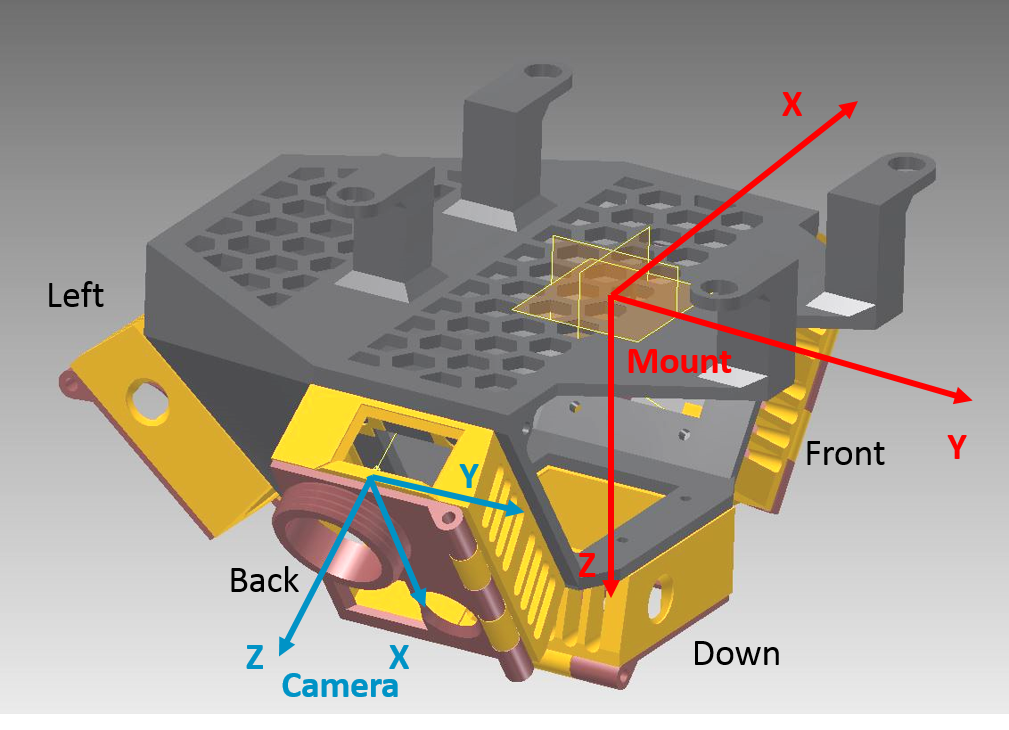
\includegraphics[scale = 0.4]{../figures/orient.png}
		\caption{The camera coordinate systems defined from the CAD model are relative to the mount coordinate system, which is defined as an arbitrary point on the top center of the mount.}
		\label{fig:orient}
	\end{figure}
	
% Table generated by Excel2LaTeX from sheet 'Sheet2'
\begin{table}[htbp]
	\centering
	\caption{The rotation and translation from the camera coordinates to the mount coordinates is defined in a right hand coordinate system where Yaw, Pitch, and Roll are defined as right hand rotations about the Z,Y, and X axes respectively.}
	\begin{tabular}{lcrrrrrr}
		\toprule
		Camera Name & Lens (mm) & Yaw($\Psi $) & Pitch($\Theta$) & Roll($\Phi$) & X (in) & Y (in) & Z (in) \\
		\midrule
		\multicolumn{1}{l}{Back} & 2.9   & 0\degree     & 55\degree    & 0\degree     & 2.74 & 0.904 & -0.931 \\
		\multicolumn{1}{l}{Down} & 5.4   & -90\degree   & 0\degree     & 0\degree     & -0.404 & 1.014 & -2.587 \\
		\multicolumn{1}{l}{Front} & 2.9   & 0\degree     & -55\degree   & 0\degree     & -2.085 & 0.904 & -1.867 \\
		\multicolumn{1}{l}{Left} & 2.9   & 180\degree   & 0\degree     & 40\degree    & -0.571 & 3.558 & -1.92 \\
		\bottomrule
	\end{tabular}%
	\label{tab:imRotations}%
\end{table}%
\begin{align}
\label{eqn:rot}
X_{mount} = R\times X_{camera} + T \\ 
\nonumber
R = DCM(\Psi,\Theta,\Phi)
\quad
T = \begin{bmatrix}
X \\ Y \\ Z
\end{bmatrix}
\end{align}

	\section{Possible Improvements}
	\subsection{Reduce Weight}
	The current sensor design weights about 700g, but not much optimization in the design for weight reduction has been performed.  If there is a large potential benefit that could be gained from a reduction in weight, the current mount and designs have some room to remove material while maintaining rigidity.  An alternative method, while more intensive, would be to incorporate carbon fiber or some other material onto the 3D printed parts to increase rigidity.  
	\subsection{Implement Weatherproofing}
	Sand or moisture can currently get into the electronics enclosure through the honeycomb pattern on the top of the mount.  If this becomes a noticeable issue, the mount should be redesigned to seal off this opening. This could be achieved with something as simple as tape across the gaps, or by adding a thin layer in the CAD design.  If the sensor is to be used in harsher environments, it could be redesigned with gaskets and more robust sealing mechanism to become more fully weatherproof.
	\subsection{Improve Panel}
	The first version of the panel contains various lights and LEDs to keep the user knowledgeable on the status of the sensor.  This panel could be modified to either add or remove status leds, or even a small LCD screen for text status updates.  If the status lights and LCDs are determined to not be useful, `improvement' could actually mean removing some components.
	\subsection{Improve Vibration Damping}
	The vibration damping implemented is a first cut, low cost approach to attempt to remove the vibration from the system.  If this method is not adequate, further investigation into vibration damping systems will need to be performed.  The design of the mount is modular enough that the only changes would be to the Legs of both the X8 bracket and the mount.  